%\section{$\Psp$-hardness of timeline-based planning with future rules and intervals $\{0,a\}$ and $\{b,+\infty)$\label{sec:pspace}}
\section[Future TP, simple trigger rules, non-singular intervals: hardness]{Future TP with simple trigger rules and non-singular intervals: hardness\label{sec:pspace}}

In this section, we first consider the future TP problem with simple trigger rules and non-singular intervals, and prove that it is $\EXPSPACE$-hard by a polynomial-time reduction from the \emph{domino-tiling problem for grids with rows of single exponential length} (it has already been presented in Section~\ref{sec:BEhard}), which is known to be  $\EXPSPACE$-complete~\cite{harel92}. Since the reduction is standard, we refer the reader to Appendix~\ref{sec:EXPSPHardFutTP} for the details of the construction.

\begin{theorem}\label{theorem:EXPSPlowerBound} 
The future TP problem, even with \emph{one state variable}, with simple trigger rules and non-singular intervals is $\EXPSPACE$-hard (under polynomial-time reductions).
\end{theorem}
By putting together Theorem~\ref{theorem:UpperBounds}, $\EXPSPACE$-completeness follows.

We now focus on the case 
%of TP with simple trigger rules and 
with intervals in $\Intv_{(0,\infty)}$, proving that the problem is $\Psp$-hard (and thus $\Psp$-complete by Theorem~\ref{theorem:UpperBounds}) by reducing periodic SAT to it in polynomial time.

The problem \emph{periodic SAT} is defined as follows~\cite{Pap94}.
We are given a Boolean formula $\varphi$ in \emph{conjunctive normal form},
defined over two sets of variables, $\Gamma=\{x_1,\ldots, x_n\}$ and $\Gamma^{+1}=\{x_1^{+1},\ldots , x_n^{+1}\}$, namely,
\[
    \varphi = \bigwedge_{t=1}^m \Big(\smashoperator[r]{\bigvee_{x\in (\Gamma \cup \Gamma^{+1})\cap L^+_t}}\quad x  \vee \smashoperator[r]{\bigvee_{x\in (\Gamma \cup \Gamma^{+1})\cap L^-_t}}  \neg x\;\Big),
\]
where $m$ is the number of conjuncts of $\varphi$ and, for $1\leq t\leq m$, $L^+_t$ (resp., $L^-_t$) is the set of variables occurring non-negated (resp., negated) in the $t$-th conjunct of $\varphi$.
%
Moreover, the formula $\varphi^j$, for $j\in\Nat\setminus\{0\}$, is defined as $\varphi$ in which we replace each variable
$x_i\in \Gamma$ by a fresh one $x_i^j$, and $x_i^{+1}\in \Gamma^{+1}$ by $x_i^{j+1}$.
Periodic SAT is then the problem of deciding the satisfiability of the (infinite-length) formula 
\[\Phi= \bigwedge_{j\in\Nat\setminus\{0\}} \varphi^j,\] that is, deciding the existence 
of a truth assignment of (infinitely many) variables $x_i^j$, for $i=1,\ldots, n,\, j\in\Nat\setminus\{0\}$, satisfying $\Phi$.

Periodic SAT is $\Psp$-complete~\cite{Pap94}; in particular membership to such a class is proved by showing that one can equivalently check the satisfiability of the (finite-length) formula $\Phi_f= \bigwedge_{j= 1}^{2^{2n}+1} \varphi^j$. Intuitively, $2^{2n}$ is the number of possible truth assignments to variables of $\Gamma\cup \Gamma^{+1}$, thus, after $2^{2n}+1$ copies of $\varphi$, we can find a repeated assignment: from that point, we can just loop through the previous assignments. 

We now %prove that future TP with simple trigger rules and intervals $\{0,a\}$, with $a\in\Nat^+$, and $\{b,+\infty[$, with $b\in\Nat$, is $\Psp$-hard by 
reduce periodic SAT to our problem.
Hardness also holds when only a single state variable is involved, and also restricting to intervals of the form $[0,a]$.

\begin{theorem}\label{theorem:PSPlowerBound} 
The future TP problem, even with \emph{one state variable}, with simple trigger rules and intervals $[0,a]$, $a\in\Nat\setminus\{0\}$, is $\Psp$-hard  (under polynomial-time reductions).
\end{theorem}
\begin{proof}
Let us define the state variable $y=(V,T,D)$, where 
\begin{itemize}
    \item $V=\{\$,\tilde{\$},stop\}\cup \{x_i^\top,x_i^\bot, \tilde{x_i}^\top, \tilde{x_i}^\bot \mid i=1,\ldots, n\}$,
    \item $T(\$)=\{x_1^\top,x_1^\bot\}$, $T(\tilde{\$})=\{\tilde{x_1}^\top, \tilde{x_1}^\bot\}$ and $T(stop)=\{stop\}$,
    \item for $i=1,\ldots, n-1$, $T(x_i^\top)=T(x_i^\bot)=\{x_{i+1}^\top,x_{i+1}^\bot\}$,
    \item for $i=1,\ldots, n-1$, $T(\tilde{x_i}^\top)=T(\tilde{x_i}^\bot)=\{\tilde{x_{i+1}}^\top,\tilde{x_{i+1}}^\bot\}$,
    \item $T(x_n^\top)=T(x_n^\bot)=\{\tilde{\$},stop\}$,
    \item $T(\tilde{x_n}^\top)=T(\tilde{x_n}^\bot)=\{\$,stop\}$, and
    \item for all $v\in\ V$, $D(v)=[2,+\infty[$.
\end{itemize}
%
Intuitively, we represent an assignment of variables $x_i^j$ by means of a timeline for $y$:
after every occurrence of the symbol $\$$, $n$ tokens are present, one for each $x_i$, and the value $x_i^\top$ (resp., $x_i^\bot$) represents a positive (resp., negative) assignment of $x_i^j$, for some \emph{odd} $j\geq 1$. Then, there is an occurrence of $\tilde{\$}$, after which $n$ more tokens occur, again one for each $x_i$, and the value $\tilde{x_i}^\top$ (resp., $\tilde{x_i}^\bot$) represents a positive (resp., negative) assignment of $x_i^j$, for some \emph{even} $j\geq 2$.
See Figure~\ref{fig:phij} for an example.
\begin{figure}[t]
    \centering
    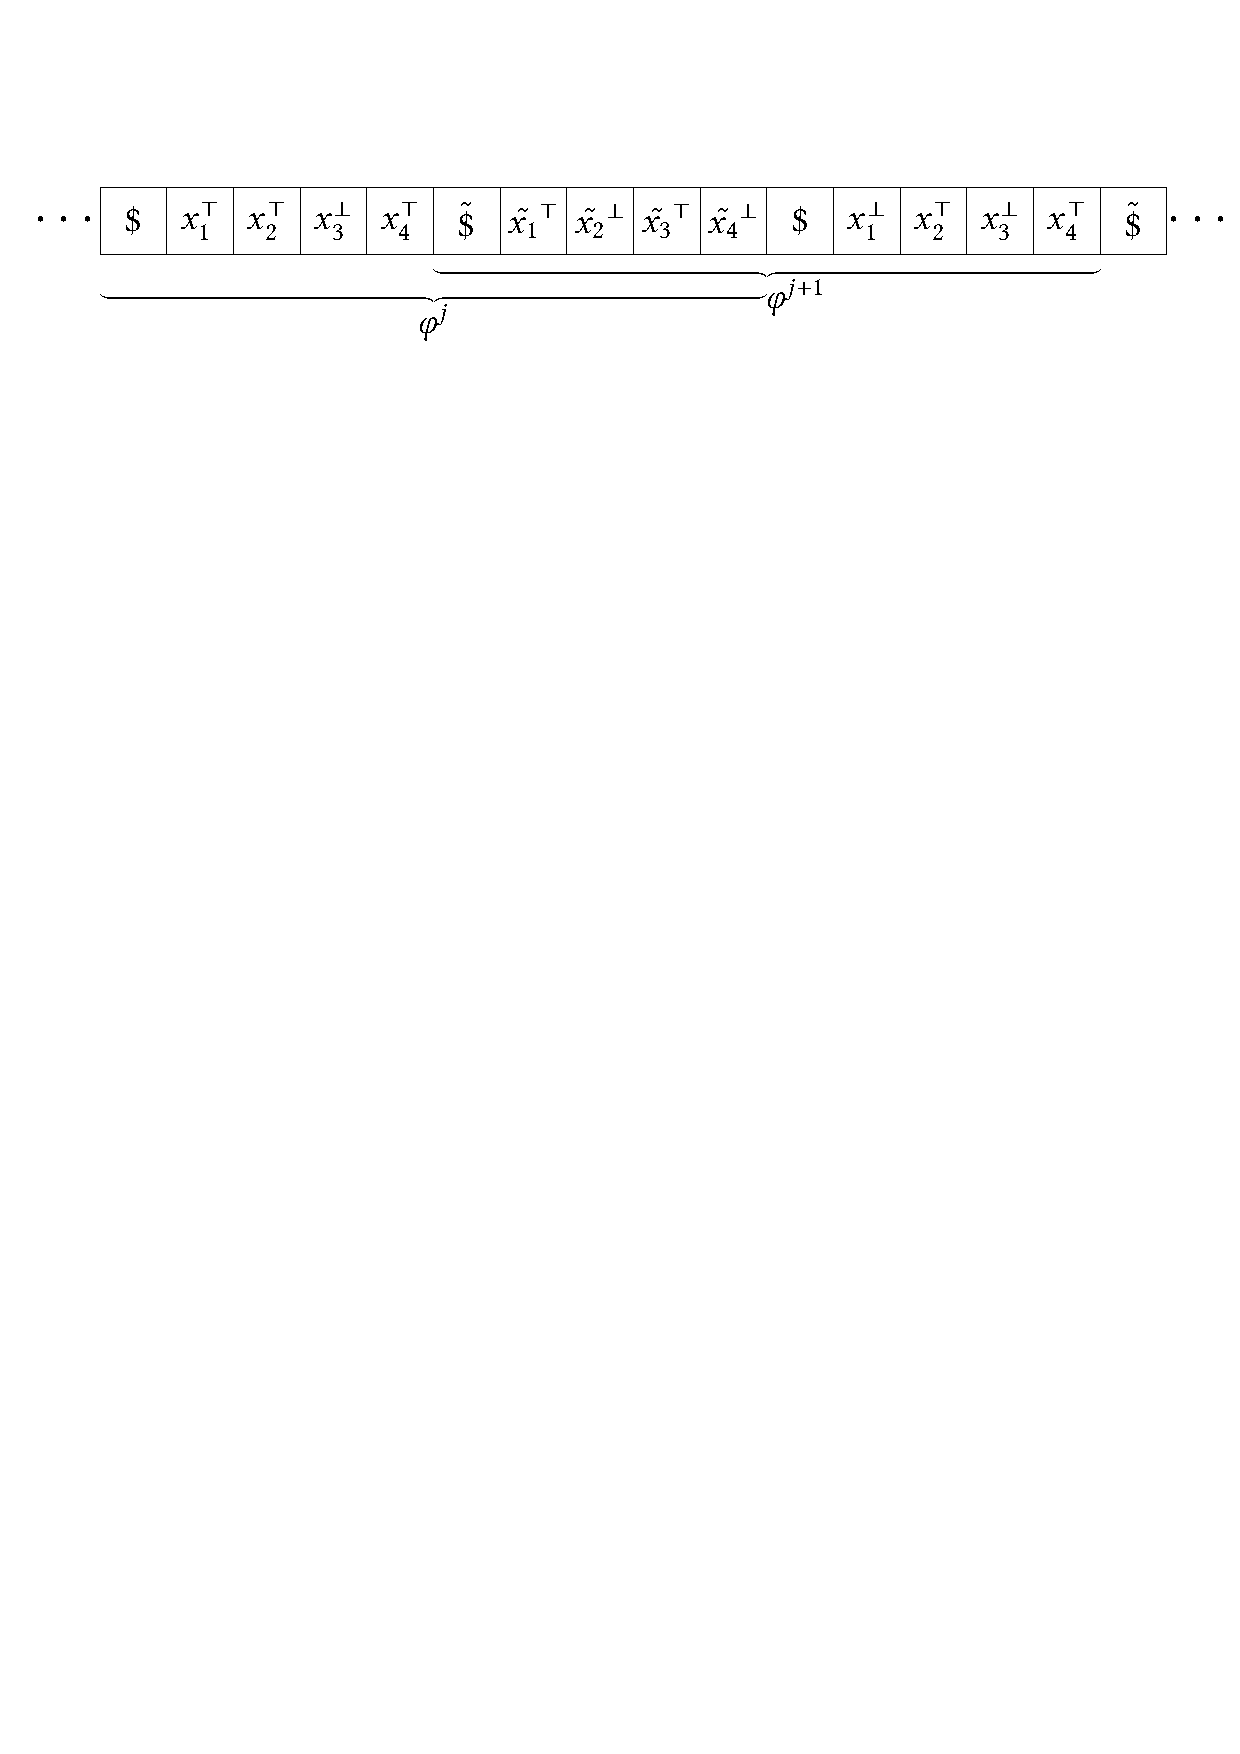
\includegraphics[width=\textwidth]{Chaps/Timelines/Psp.pdf}
    \caption{Let
    the formula $\varphi$ be defined over two sets of variables, $\Gamma=\{x_1,x_2,x_3,x_4\}$ and $\Gamma^{+1}=\{x_1^{+1},x_2^{+1},x_3^{+1},x_4^{+1}\}$. 
    The $j$-th copy (we assume $j$ is odd) of $\varphi$, i.e., $\varphi^j$, is satisfied by the assignment $x_1^j\mapsto \top$, $x_2^j\mapsto \top$, $x_3^j\mapsto \bot$, $x_4^j\mapsto \top$, $x_1^{j+1}\mapsto \top$, $x_2^{j+1}\mapsto \bot$, $x_3^{j+1}\mapsto \top$, $x_4^{j+1}\mapsto \bot$. The analogous for $\varphi^{j+1}$. }
    \label{fig:phij}
\end{figure}

We start with the next simple trigger rules, one for each $v\in V$: 
\[o[y=v]\to o\leq^{\mathsf{s},\mathsf{e}}_{[0,2]} o.\]
Paired with the constraint function $D$, they enforce
all tokens' durations to be \emph{exactly} 2: intuitively, since we exclude singular intervals, requiring, for instance, that a token $o'$ starts  $t$ instants of time after the end of $o$, with $t\in [\ell,\ell+1]$ and even $\ell\in\Nat$, boils down to $o'$ starting \emph{exactly} $\ell$ instants after the end of $o$. We also observe that, given the constant token duration, the density of the time domain does not play any role in this proof.

We now add the next rules:
\begin{itemize}
\item
    $\true \to \exists o[y=\$]. o\geq^{\mathsf{s}}_{[0,1]} 0$;
\item
    $\true \to \exists o[y=\tilde{\$}]. o\geq^{\mathsf{s}}_{[0,1]} (2^{2n}+1)\cdot 2(n+1)$;
\item
    $\true \to \exists o[y=stop]. o\geq^{\mathsf{s}}_{[0,1]} (2^{2n}+2)\cdot 2(n+1)$.
\end{itemize}
They respectively impose that $(i)$~a token with value $\$$ starts exactly at $t=0$ (recall that the duration of every token is 2);
$(ii)$~there exists a token with value $\tilde{\$}$ starting at $t=(2^{2n}+1)\cdot 2(n+1)$; 
$(iii)$~a token with value $stop$ starts at $t=(2^{2n}+2)\cdot 2(n+1)$. 
We are forcing the timeline to encode truth assignments for variables $x_1^1,\ldots, x_n^1,\ldots, x_1^{2^{2n}+2} ,\ldots , x_n^{2^{2n}+2}$: as a matter of fact, we will decide satisfiability of the finite formula $\Phi_f= \bigwedge_{j= 1}^{2^{2n}+1} \varphi^j$, which is equivalent to $\Phi$.

% The following rules require that, after a token with value $\$$ (resp., $\tilde{\$}$), there is a token with value $\tilde{\$}$ (resp., $\$$) or $stop$, after exactly $2n$ instants of time (recall that the transition function forces the presence of a token for each $x_i^j$ between near occurrences of $\$$/$\tilde{\$}$). 
% \[
%     a[y=\$]\to (\exists b[y=\tilde{\$}]. a\leq ^{\mathsf{e},\mathsf{s}}_{[0,2n]} b) \vee (\exists b[y=stop]. a\leq ^{\mathsf{e},\mathsf{s}}_{[0,2n]} b).
% \]
% \[
%     a[y=\tilde{\$}]\to (\exists b[y=\$]. a\leq ^{\mathsf{e},\mathsf{s}}_{[0,2n]} b) \vee (\exists b[y=stop]. a\leq ^{\mathsf{e},\mathsf{s}}_{[0,2n]} b).
% \]

We now consider the next rules, that enforce the satisfaction of each $\varphi^j$ or,
equivalently, of $\varphi$ over the assignments of $(x_1^j,\ldots, x_n^j, x_1^{j+1},\ldots, x_n^{j+1})$.

For the $t$-th conjunct of $\varphi$, % $1\leq t\leq m$, 
we define the future simple rule:
\begin{multline*}
    o[y=\tilde{\$}]\to \\
    \Big(\smashoperator{\bigvee_{x_i\in \Gamma\cap L^+_t}} \exists o'[y=\tilde{x_i}^\top]. o\leq ^{\mathsf{e},\mathsf{s}}_{[0,4n]} o' \Big) \vee 
        \Big(\smashoperator{\bigvee_{x_i^{+1}\in \Gamma^{+1}\cap L^+_t}} \exists o'[y=x_i^\top]. o\leq ^{\mathsf{e},\mathsf{s}}_{[0,4n]} o' \Big) \vee \\
        \Big(\smashoperator{\bigvee_{x_i\in \Gamma\cap L^-_t}} \exists o'[y=\tilde{x_i}^\bot]. o\leq ^{\mathsf{e},\mathsf{s}}_{[0,4n]} o' \Big) \vee 
        \Big(\smashoperator{\bigvee_{x_i^{+1}\in \Gamma^{+1}\cap L^-_t}} \exists o'[y=x_i^\bot]. o\leq ^{\mathsf{e},\mathsf{s}}_{[0,4n]} o' \Big) \vee \\
        \exists o''[y=stop]. o\leq ^{\mathsf{e},\mathsf{s}}_{[0,2n]} o''.
\end{multline*}
Basically, this rule (the rule where the trigger has value $\$$ being analogous) states that, after every occurrence of $\tilde{\$}$, a token $o'$, making true at least a (positive or negative) literal in the conjunct, must occur by $4n$ time instants (i.e., before the following occurrence of $\tilde{\$}$).
The disjunct $\exists o''[y=stop]. o\leq ^{\mathsf{e},\mathsf{s}}_{[0,2n]} o'' $ is present just to avoid evaluating $\varphi$ on the $n$ tokens before (the first occurrence of) $stop$.

%To conclude the proof we observe that the state variable 
The variable $y$ and all synchronization rules can be generated in time polynomial in $|\varphi|$ (in particular, all interval bounds and time constants of time-point atoms have a value, encoded in binary, in $O(2^{2n})$).
\end{proof}

By Theorem~\ref{theorem:UpperBounds} and Theorem~\ref{theorem:PSPlowerBound}, $\Psp$-completeness of 
future TP with simple trigger rules and intervals in $\Intv_{(0,\infty)}$ follows.

In the next section we focus on a different restriction of the TP problem, which will allow us to devise a $\NP$ planning algorithm for it.